As compute capabilities continue to outpace I/O capacity on supercomputers, \textit{in situ} processing is an increasingly important solution to enable analysis of large-scale simulation data~\cite{bauer2016situ}.
%
It can take the form of (1) direct analysis or visualization if a priori knowledge of the desired task exists, or (2) a data reduction routine to support exploratory use cases (i.e., no a priori knowledge). 
%
In situ processing involves coupling with the simulation code and operating on data as it is generated. 
% in either a tightly-coupled (utilize same resources) or loosely-coupled (distinct resources) setting.
%In situ processing involves operating on simulation data as it is generated in either a tightly-coupled (utilize same resources) or loosely-coupled (distinct resources) setting.
%
A benefit of operating in situ is access to the full spatiotemporal resolution of the simulation data in memory.
%
However, in situ analysis tasks operate in constrained environments and are afforded limited execution time and memory.
%
Further, these analysis tasks often have execution time constraints and must scale effectively since simulations execute across hundreds of compute nodes~(CNs).
%
%Thus, investigating the overhead in situ processing introduces is critical.
%
In this paper, we investigate the performance of in situ data reduction via Lagrangian analysis to enable time-varying vector field analysis.
%In this paper, we investigate the performance of an in situ data reduction routine to enable time-varying vector field analysis.
%
%Specifically, we consider the computation of Lagrangian flow maps.
\begin{figure}[!t]
\centering
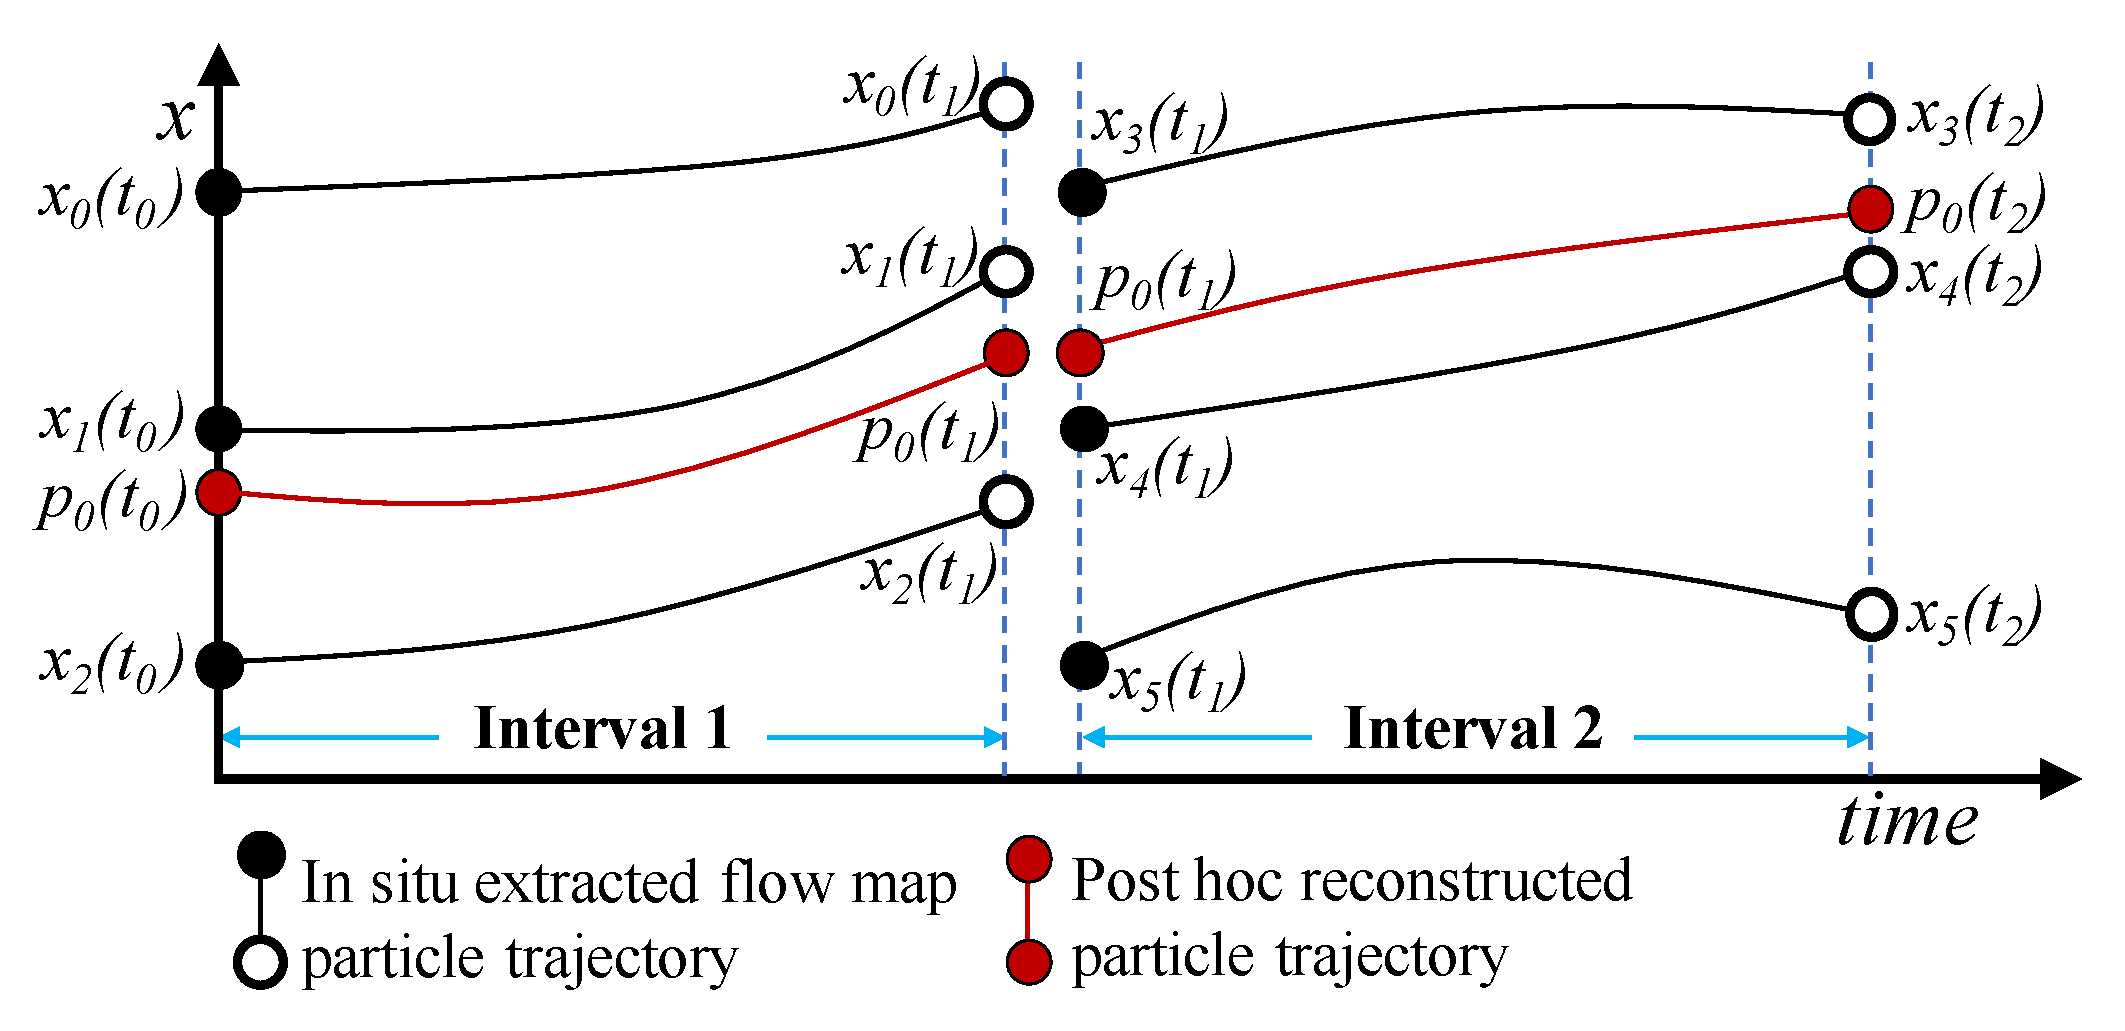
\includegraphics[width=\linewidth]{Images/phases_new_tall.pdf}
\caption{\fix{The phases of Lagrangian analysis. The in situ phase uses uniform seed placement and extracts flow maps over temporally nonoverlapping intervals. The extracted flow maps are used as input during the post hoc phase. In this example, the red particle's trajectory is calculated by interpolating the flow maps over two intervals of time, i.e., $p_0$ is interpolated from $x_1$ and $x_2$ in the first time interval and $x_3$ and $x_4$ in the second time interval.}}
\vspace{-6mm}
\label{fig:phases}
\end{figure}


Lagrangian analysis is a powerful tool to explore time-varying vector fields generated by simulations.
%, and it is widely used for climate modeling.
%, and is extensively used forocean circulation models~\cite{VANSEBILLE201849}. 
%
The notion of calculating a Lagrangian flow map, i.e., sets of particle trajectories, for an ocean modeling simulation ``online" for ``offline'' exploration was first proposed by Vries et al.~\cite{vries2001calculating} two decades ago.
%
More recently, compared to the traditional Eulerian technique under sparse temporal settings, Agranovsky et al.~\cite{agranovsky2014improved} evaluated reduced Lagrangian representations of time-varying vector fields and showed significantly improved accuracy-storage propositions for exploration. 
%compared to the traditional Eulerian technique under sparse temporal settings. 
%
%The Lagrangian representation consists of particle trajectories that are computed using every cycle of a simulation. 
Figure~\ref{fig:phases} illustrates the approach.
%
The Lagrangian flow maps 
%(denoted by F$X$$\rightarrow$$Y$ in Figure~\ref{fig:phases}) 
are computed in situ using every cycle of a simulation, i.e., the full temporal resolution.
%
After calculating and storing the flow maps, post hoc analysis tasks can use the flow maps to interpolate new particle trajectories to explore the vector field.
%
%


The Agranovsky et al.~\cite{agranovsky2014improved} study has been followed by several works in the areas of generation and interpolation of Lagrangian representations~\cite{chandler2015interpolation, sane2019interpolation, rapp2019void, jakob2020fluid}, theoretical and empirical error analysis~\cite{bujack2015lagrangian, chandler2016analysis, hummel2016error, sane2018revisiting}, and use of reduced data sets for ocean modeling applications~\cite{envirvis.20171099}.
%
Although these works advance our understanding of the technique at a theoretical level, the scalability of the technique has not been previously addressed. 
%
%the current literature lacks a viability evaluation for the in situ computation of a distributed Lagrangian representation at scale on a modern supercomputer.
%Although these works advance our understanding of the technique at a theoretical level, the current literature lacks an evaluation of the in situ computation of a distributed Lagrangian representation at scale on a modern supercomputer.
%
The authors of a recent comprehensive review of Lagrangian analysis~\cite{VANSEBILLE201849}, have identified the primary challenges as (1) utilization of heterogenous computer architectures, (2) providing parallel performance and scalability, and (3) lack of an accessible API that allows integration with different simulations. 
%
In this paper, we address the challenge of scalability, as well as utilize a runtime in situ infrastructure for multiphysics HPC simulations and GPUs for Lagrangian flow map computation. 

With this study, our contributions include:
\vspace{-1mm}
\begin{itemize}[leftmargin=*,noitemsep,topsep=0pt,parsep=0pt,partopsep=0pt]
\item A scalability study of distributed-memory particle advection using GPUs for Lagrangian flow map computation. 
\item An evaluation of a proposed performance optimization, i.e., computing local Lagrangian flow maps, across multiple extraction parameter configurations.
%\item An identification of the differing constraints/requirements of distributed-memory particle advection for in situ Lagrangian flow map extraction versus post hoc analysis.
\vspace{-1mm}
\end{itemize}

%Computing a Lagrangian flow map in a practical in situ environment is hard since it involves performing distributed-memory particle advection under in situ constraints. 
%
%Efficient distributed-memory particle advection is challenging and has been extensively researched, with studies typically producing strategies to improve scalability or load balance~\cite{surveys}.
%

%The first part of the paper discusses work related to the use of Lagrangian flow maps to enable time-varying flow visualization and relevant distributed-memory particle advection research conducted for post hoc analysis. 
%
%Next, we give an overview of the in situ computation process, followed by our rationale for computing local Lagrangian flow maps.
%
%Section~\ref{sec:study} describes the experiments, and Section~\ref{sec:results} demonstrates the applicability and viability of the method using multiple data sets.
%
%Various aspects of the evaluated technique and possible future works are discussed in Section~\ref{sec:discussion}.
%
%Finally, we draw conclusions from our study in Section~\ref{sec:conclusion}.


%We compare distributed-memory particle advection in the contexts of in situ data reduction and post hoc analysis in Section~\ref{}.
%
%Next, we provide details of our implementation, the specific in situ infrastructure we utilize, and propose a simple optimization in Section~\ref{}.
%
%Our optimization involves computing local flow maps that address scalability concerns while maintaining relatively high reconstruction accuracy.
%
%Sections~\ref{} and~\ref{} provide details of the experiments and results analyzing scalability and reconstruction accuracy.
%
%Finally, Sections~\ref{} covers a discussion of current limitations and future directions of research, while Section~\ref{} concludes this paper.
%

